\documentclass[language=german,style=exam]{smo}

\usepackage{tikz}

\title{SMO - Vorrunde}

\begin{document}

\begin{enumerate}

\item[\textbf{1.}] 
An der SMO-Strasse stehen $n$ Häuser mit den Hausnummern 1 bis $n$, wobei $n$ eine natürliche Zahl ist. Die Häuser mit den ungeraden Nummern stehen dabei auf der linken Strassenseite, die Häuser mit den geraden Nummern auf der rechten. Der Postbote Quirin möchte jedem Haus eine Zeitung vorbeibringen. Wie viele Möglichkeiten hat er, dies zu tun, wenn er nach jeder abgegebenen Zeitung die Strassenseite wechseln möchte?

\bigskip

\item[\textbf{2.}] 
Für welche natürlichen Zahlen $n$ ist es möglich, ein $n\times n$ Feld lückenlos und überlappungsfrei mit T-Tetrominos und einer ungeraden Anzahl an Square-Tetrominos zu bedecken?
\vspace{-0cm}
\begin{center}
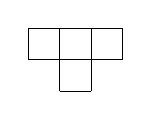
\begin{tikzpicture}[scale=0.4]
\draw (0,1) grid (3,2);
\draw (1,0) grid (2,1);
\end{tikzpicture}
\quad
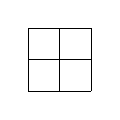
\begin{tikzpicture}[scale=0.4]
\draw (0,0) grid (2,2);
\end{tikzpicture}
\end{center}
\textit{Bemerkung: Es ist erlaubt, keine T-Tetrominos zu verwenden.}
\vspace{0.2cm}
\item[\textbf{3.}]
Finde alle Tripel $(a,b,c)$ natürlicher Zahlen, sodass
\[
\frac{a+b}{c},\frac{b+c}{a},\frac{c+a}{b}
\]
%\[
%c \,|\, a+b \qquad a \,|\, b+c \qquad b \,|\, a+c
%\]
ebenfalls natürliche Zahlen sind.

\bigskip

\item[\textbf{4.}] 
Sei $ABC$ ein spitzwinkliges Dreieck und $W$ der Schnittpunkt der Winkelhalbierenden von $\angle ACB$ und der Seite $AB$. Weiter seien $I_A$ und $I_B$ die Inkreismittelpunkte der Dreiecke $AWC$ respektive $WBC$. Die Geraden $I_AW$ und $I_BB$ schneiden sich im Punkt $D$. Sei $M$ der Mittelpunkt der Strecke $DI_B$.
Zeige, dass $MWBC$ ein Sehnenviereck ist.

\textit{Bemerkung: Die drei Winkelhalbierenden eines Dreiecks schneiden sich in einem Punkt, dem Inkreismittelpunkt.}

\bigskip

\item[\textbf{5.}] 
Den unten abgebildeten Spielstein nennen wir eine Treppe. Für welche Paare $(m,n)$ natürlicher Zahlen mit $m,n\geq 6$ ist es möglich, ein $m\times n$ Feld lückenlos und überlappungsfrei mit Treppen zu bedecken?
\vspace{-0cm}
\begin{center}

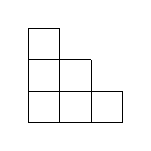
\begin{tikzpicture}[scale=0.4]
\draw (-1,0) grid (2,1);
\draw (-1,1) grid (1,2);
\draw (-1,2) grid (0,3);
\end{tikzpicture}
\quad
\end{center}

\bigskip

\end{enumerate}

\vspace{1cm}

\center{\hspace{1cm} Viel Glück!}
\end{document}
